\chapter{Lösen von ODEs mittels stückweiser Linearisierung}

\section{Verallgemeinerte Mittelpunktsregel}

Unser Ziel ist es nun, ausgehend von der wohlbekannten Impliziten Mittelpunktsregel
\[
 \xhat  = \xcheck + hF\left( \frac{\xhat + \xcheck}{2}\right)
\]
die im vorherigen Kapitel hergeleitete stückweise Linearisierung zur Lösung von ODEs mit verketteter stückweise glatter rechter Seiten anzuwenden.
Hierbei ist $\xhat = x(h)$ und $\xcheck = x(0)$.

Gegeben sei eine gewöhnliche Differentialgleichung
\[
 \dot x = F(x(t))
\]
mit verkettetem stückweise glattem und global Lipschitzstetigem $F$. Mit dem Hauptsatz der Differential- und Integralrechnung folgt
\[
 \xhat - \xcheck = \int_0^h F(x(t)) \text{d}t
\]
und mit $t = \frac{h}{2} + \tau h$ als Substitution ergibt sich
\[
 \xhat - \xcheck = h\int_{-\sfrac{1}{2}}^{\sfrac{1}{2}} F\left(x \left(\sfrac{h}{2} + \tau h\right)\right) \text{d}\tau
\]
Da das Integral in den Grenzen $-\sfrac{1}{2}$ und $\sfrac{1}{2}$ liegt, stellt $\sfrac{h}{2}$ den Mittelpunkt des Integrationsgebietes dar. Durch Approximation von $x(t)$ durch die Sekante $(\frac{1}{2} - \tau) \xcheck + (\frac{1}{2} + \tau) \xhat$ folgt:
\[
 \begin{aligned}
 \xhat - \xcheck & = h\int_{-\sfrac{1}{2}}^{\sfrac{1}{2}} F\left(\frac{\xcheck + \xhat}{2} + \tau (\xhat - \xcheck)\right) \text{d}\tau + \mathcal O(h^3)
 \end{aligned}
\]
Nun schätzen wir die rechte Seite $F(\ldots)$ durch seine stückweise Linearisierung ab und erhalten schließlich
\[
 \xhat -  \xcheck = h\int_{-\sfrac{1}{2}}^{\sfrac{1}{2}} F(\xo) + \Delta F(\xo;\tau (\xhat - \xcheck))  \text{d}\tau + \mathcal O(h^3)
\]
die von Griewank in \cite[S.21 (14)]{monster} eingeführte verallgemeinerte Implizite Mittelpunktsregel
\begin{equation}
 \xhat -  \xcheck = h\int_{-\sfrac{1}{2}}^{\sfrac{1}{2}} F(\xo) + \Delta F(\xo;\tau (\xhat - \xcheck))  \text{d}\tau
\end{equation}

Da sowohl die Approximation durch Sekanten als auch der stückweisen Linearisierung einen Fehler von $\mathcal O(h^2)$ bzgl. der exakten Lösung $x(t)$ besitzen und das Integral $h$ als Multiplikator besitzt ergibt sich letztendlich ein Fehler dritter Ordnung.

Der Vorteil der Formel besteht darin, dass sie konsistent zur Impliziten Mittelpunktsregel ist. Falls $F$ nämlich glatt ist, so kommt die Auswertungsprozedur für $\Delta F(\xo;\tau (\xhat - \xcheck))$ ohne die Regel \eqref{eq:absAdRule} aus und es gilt 
\[
 \Delta F(\xo;\tau (\xhat - \xcheck)) = F'(\xo) \tau (\xhat - \xcheck)
\]
Das bedeutet, dass
\[
\begin{aligned}
   \xhat -  \xcheck &= h\int_{-\sfrac{1}{2}}^{\sfrac{1}{2}} F(\xo) + \Delta F(\xo;\tau (\xhat - \xcheck))  \text{d}\tau\\
		    &= h\int_{-\sfrac{1}{2}}^{\sfrac{1}{2}} F(\xo) + F'(\xo)\tau (\xhat - \xcheck))  \text{d}\tau\\
		    &= h F(\xo)
\end{aligned}
\]
Damit ist die verallgemeinerte Implizite Mittelpunktsregel eine echte Verallgemeinerung der bekannten Impliziten Mittelpunktsregel. 
Griewank bewies in \cite[Prop.4]{monster} ihre Konvergenzeigenschaft
\begin{theorem}[Konvergenz verallg. Impl. Mittelpunktsregel]
 Angenommen, $F$ sei eine verkettete stückweise glatte Funktion und Lipschitzstetig in einer offenen Umgebung $\mathcal D$ des Ursprungs $\xcheck =0$. Dann existiert eine obere Schranke $\bar h>0$, sodass für alle $h<\bar h$ die Funktion 
 \[
    hG(x) = h\int_{-\sfrac{1}{2}}^{\sfrac{1}{2}} F(\xo) + \Delta F(\xo;\tau (\xhat - \xcheck))  \text{d}\tau
 \] 
 eine abgeschlossene Kugel $B_\rho(0)\subset \mathcal D$, $\rho>0$ in sich selbst abbildet und kontraktiv ist.
 Desweiteren genügt der eindeutige Fixpunkt $x_h\in B_\rho(0)$
 \[
  x_h - x(h) = \mathcal O(h^3)
 \]
  wobei $x(t)$ die Gleichung $\dot x(t) = F(x(t))$ mit  $x(0)= 0$ löst.
\end{theorem}

Für den von Boeck \cite{boeck14} hergeleiteten Algorithmus benötigen wir zum einen die Möglichkeit eine stückweise lineare Funktion möglichst genau in einem Intervall zu integrieren als auch ein Löser für Lineare Gleichungssysteme.
% Dies wird im nächsten Abschnitt behandelt.

\section{Quadratur und Unfoldeded Newton}
\subsection{Quadraturverfahren}

Die Aufgabe besteht nun darin, eine stückweise lineare Funktion $F:\R^n \to \R^m$ genau zu integrieren. Dazu sei die stückweise Linearisierung $F(\xo) + \Delta F(\xo,\Delta x)$ mit einer Richtung $\Delta x$ als Abs-Normal Form gegeben, wie sie in Abschnitt \ref{sec:absNormalForm} eingeführt wurde. 
Für unser Problem ist es ausreichend, nur $\Delta F(\xo,\Delta x)$ zu betrachten, da $F(\xo)$ konstant ist.
Nehmen wir an, das in dem Integrationsgebietes des Integrals
\begin{equation}
\label{eq:quadInitialProblem}
 \int_0^{\sfrac{1}{2}} \Delta F(\xo,t\Delta x) \text{d}t
\end{equation}
$k$ Kinks des Integranten vorhanden sind. 
%Kink Berechnung
Um diese Kinks aus der Abs-Normal Form zu berechnen, werden die switching Variablen $z_j$, $j=1,\dots,s$ aus der Abs-Normal Form betrachtet. Wie bereits in Kapitel \ref{sec:absNormalForm} erwähnt sind diese Werte für sich genommen stückweise affine Funktionen, an deren Nullstellen ein Kink auftritt,
d.h. an ihren Nullstellen findet ein Vorzeichenwechsel statt. Um zu wissen, wie weit wir von einem Punkt $\xo$ in Richtung $\Delta x$ gehen können bis wir solch eine Nullstelle erreichen, wollen wir diese \textit{kritischen Multiplikatoren} $\tau_j$, $j=1,\ldots, s$ berechnen. 
%Quadraturbeschreibung blub
\begin{figure}[H]
\centering
 \documentclass{standalone}
\usepackage{pgfplots,pgfplotstable}

\usetikzlibrary{external}

\begin{document}

\tikzsetnextfilename{multiple_kinks}
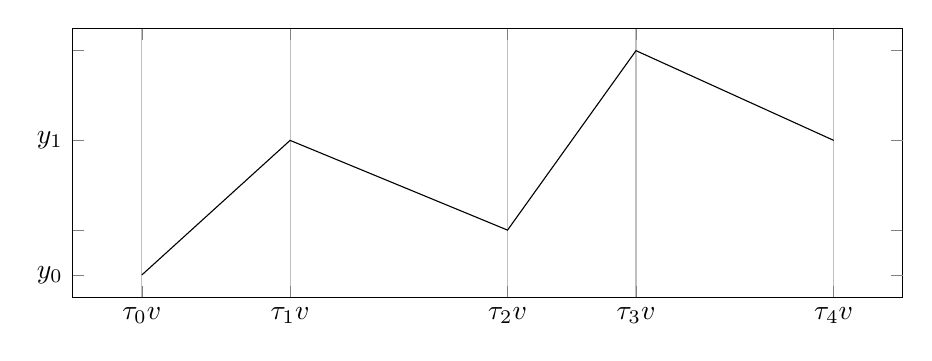
\begin{tikzpicture}
% \draw (0,0) grid (7,3);
% \draw[help lines,->] (0,0) -- (7,0) node[anchor=north west] {$v$};
% \draw[help lines,->] (0,0) -- (0,3) node[anchor=south east] {$y$};
% 
% \draw (0,1) -- (1,2) -- (2,0.5) -- (3,1.5) -- (4,1) -- (5,2.5) -- (6,2);
\begin{axis}[
	width=\textwidth,
	height=5cm,
% 	xlabel = $v$,
% 	ylabel = $y$,
	xtick = data,
	ytick = data,
	xmajorgrids,
	xticklabel={$\tau_{\pgfmathprintnumber{\ticknum}}v$},
	yticklabel=\empty,
	extra y ticks={1,1.3},
	extra y tick labels={$y_0$,$y_1$},
]
	\addplot[no marks] table {
		0 1
		1.5 1.3
		3.7 1.1
		5 1.5
		7 1.3
	};
\end{axis}

\end{tikzpicture}

 
\end{document}

 \caption{Quadratur zwischen mehreren Kinks}
\label{fig:quadrature} 
\end{figure}
Dafür nehmen wir die erste Zeile der Abs-Normal-Form \eqref{eq:absNormalForm}
\begin{equation}
\label{eq:absNormalZ}
 z = c+Zx + L|z|
\end{equation}
und deren Richtungsableitung an $z$
\begin{equation}
\label{eq:absNormalZDerivative}
 \dot z = Z\Delta x + L\Sigma \dot z, \quad
 \Sigma  = \diag(\sigma(z)) ~ \text{mit } \sigma_j =  \begin{cases}
            \sign(z_j) & \text{falls } z_j\neq 0\\
            \sign(\dot z_j) &  \text{sonst}
           \end{cases}
\end{equation}

und bilden für jedes $z_j$ seine Tangente
\[
 z_j + \tau \dot z_k = 0 \quad \Leftrightarrow \quad \tau =- \frac{z_k}{\dot z_k}
\]
deren Nullstelle wir berechnen. Da sich das Vorzeichen des Abs Aufrufs in \eqref{eq:absNormalZ} bis zur Nullstelle nicht ändert, wir uns also im selben Polyeder befinden, haben wir lokal eine affine Funktion, deren Richtungsableitung \eqref{eq:absNormalZDerivative} lokal wohldefiniert ist.
Falls $z_j\dot z_j <0$ gilt, kreuzt die Tangente in Richtung $\Delta x$ einen Kink.
Der kritische Multiplikator $\tau_*$ ergibt sich dann als das Minimum der errechneten Werte oder im Falle, dass kein Kink vorhanden ist als obere Integrationsgrenze
\[
 \tau_* = \min \begin{cases}
		\frac{1}{2}\\
		\inf_j\lbrace -\frac{z_j}{\dot z_j}~ \vert ~ \dot z_j \cdot z_j <0 \rbrace
	       \end{cases}
\]

%Quadraturbeschreibung blub
\begin{figure}
\centering
 \documentclass{standalone}
\usepackage{pgfplots,pgfplotstable}

\usetikzlibrary{external}

\begin{document}

\tikzsetnextfilename{finding_kinks}
\begin{tikzpicture}[x=1.7cm,y=1.7cm]
\draw[->] (0,-.2) -- (0,2.5);
\draw[->] (-.2,0) -- (2.5,0);
\draw[] (-.2,2.2) -- (2.2,-.2) 
node[sloped,pos=0.5,anchor=north] {$z_j + \tau_j \dot z_j$};
% \draw[decorate,decoration={brace,raise=4pt}] (0,2) -- (2,0) 
% node[pos=0.5,anchor=south west] {$\tau$};
\draw[] (-.1,2) -- (.1,2);
\draw (2,-.1) -- (2,.1);
\node[] at (-.3,2) {$z_j$};
\node[pos=0,anchor=north east] {$0$};
\end{tikzpicture}

 
\end{document}

 \caption{Kink- Berechnung}
\label{fig:findingKinks} 
\end{figure}

Nun, da wir die Stellen der $k$ Kinks ausrechnen könnne, teilen wir das Intervall $[0,\frac{1}{2}]$ in $k$-Abschnitte mit reellen Zahlen $0=\tau_0<\tau_1<\ldots<\tau_k = \sfrac{1}{2}$,  sodass
\[
 [0,\sfrac{1}{2}] = \bigcup_{i=0}^{k-1} [\tau_i,\tau_{i+1}]
\]
damit wir das Integral zerlegen können in
\[
 \int_0^{\sfrac{1}{2}} \Delta F(\xo,t\Delta x) \text{d}t = \sum_{i=0}^{k-1} \int_\tau^{\sfrac{1}{2}} \Delta F(\xo,t\Delta x) \text{d}t
\]
Mit $y_i = \Delta F(\xo;\tau_i \Delta x)$ und $F$ stückweise linear folgt, dass sich die Quadratur \ref{eq:quadInitialProblem} zu
\begin{equation}
\begin{aligned}
 \int_{\tau_{i-1}}^{\tau_i} \Delta F(\xo;t\Delta x) \text{d}t &= \int_{\tau_{i-1}}^{\tau_i}\left[ y_i+ \frac{y_{i+1}-y_i}{\tau_{i+1}-\tau_i}(t-\tau_i) \right] \text{d}t \\
 &=\frac{1}{2}(\tau_{i+1} -\tau_i)(y_{i+1}-y_i)
 \end{aligned}
\end{equation}
vereinfacht, also zur Trapezregel. Für stückweise lineare Funktionen ist die eben beschriebene Integrationsmethode exakt, da die Trapezregel für lineare Funktionen exakt ist.
Mit dem Algorithmus in Prozedur \ref{alg:quad} kann nun die Quadratur für stückweise lineare Funktionen berechnet werden. 
\begin{algorithm}[H]
% \caption{Quadraturformel für stückweise lineare Funktionen}
% \label{alg:quad}
\algrenewcommand{\algorithmiccomment}[1]{\hfill{\scriptsize #1}}
\begin{algorithmic}
\Function{integrate}{$\Delta x$} 
  \State {$x \gets 0$}
  \State {$z \gets$ calculate\_z($x$)}
  \State {$dy_{old} \gets$ eval($z,x$)}
  \State {quadResult $\gets 0$}
  \State {$\tau$ $\gets 0$}
  \Repeat 
    \State {$\tau_{new} \gets \frac{1}{2}$}
    \For{$i\gets 0,\ldots,s-1$}
      \State{ $\dot z = \sum_{i=0}^{n} Z_{ij}\cdot \Delta x_j + \sum_{i=0}^s L_{ij}\Sigma \dot z_j$}
      \If{$-\frac{z_i}{\dot z_i} \in [0,\tau_{\text{new}}]$}
	\State{$\taunew \gets -\frac{z_i}{\dot z_i}$}
% 	\State{$\tau_{\text{new}} = 0.5 - \tau$}
% 	\State{\tau =0.5}
% 	\State{$\tau \gets \tau + \tau_{\text{new}}$}
      \EndIf
    \EndFor 
    \If{$\tau + \taunew < 0.5$}
      \State{$\tau_{\text{new}} = 0.5 - \tau$}
      \State{$\tau =0.5$}
    \Else
      	\State{$\tau \gets \tau + \tau_{\text{new}}$}
    \EndIf
    \State{$x\gets\tau \Delta x$}
    \State{$z \gets$ calculate\_z($x$)}
    \State{$dy \gets$ eval($z,x$)}
    \State{quadResult $\gets$ quadResult + $\sfrac{\taunew}{2}(dy_{\text{old}}+ dy)$}
    \State{$dy_{\text{old}} \gets dy$}
  \Until{$\tau > \sfrac{1}{2}$}
\EndFunction
\end{algorithmic}
\caption{Quadratur stückweise linearer Funktionen}
\label{alg:quad}
\end{algorithm}


\subsection{Verallgemeinerte Gradienten}
Die Menge der limiting Jacobians reduziert sich für unser stückweise lineares Modell zu 
\[
 \partial^L F(x) = \lbrace J_\sigma: x\in \bar S_\sigma \text{ mit }\sigma \text{ offen} \rbrace
\]

\subsection{Unfolded Newton}
Als nächstes gilt es, ein lineares Gleichungssystem zu lösen, also 
\[
 F(x) = 0
\]
zu berechnen.


% \section{Verallgemeinerte Newton}
\section{Algorithmus}

\section{Romberg Interpolation}
\cite{boeck14}
